\chapter{Povezivanje razvojnog sustava i računala}

Računalo i STM32 razvojni sustav dva su odvojena sustava koja moraju međusobno komunicirati i razmjenjivati podatke. Za ostvarenje njihove veze razvijena su dva programska rješenja:
\begin{enumerate}
	\item programska potpora za mikrokontroler, koja će omogućiti pokretanje i snimanje zvučnog zapisa te njegov prijenos BLE sučeljem,
	\item programska potpora za računalo, koja će ostvariti Bluetooth vezu između računala i mikrokontrolera te omogućiti prijem i pohranu primljenog audio signala.
\end{enumerate} 

\section{Programska potpora za mikrokontroler}

Dvije glavne funkcionalnosti koje mikrokontroler mora sadržavati su snimanje zvuka i njegov prijenos BLE komunikacijskim sučeljem. Za rad mikrokontrolera odabran je paket funkcija \textit{FP-AUD-BVLINKWB1} iz alata \textit{STM32Cube} koji je razvila tvrtka \textit{STMicroeletronics}. Ovaj \textit{firmware} omogućava potpuni dvosmjerni prijenos zvuka koji se prenosi BLE sučeljem koristeći Opus algoritam za kompresiju. Aplikacija sadrži \textit{drivere} i posrednički softver (engl. \textit{middleware}) za BLE i digitalne MEMS mikrofone. Također uključuje kompletan Opus audio kodek kao \textit{middleware} za izvođenje dvosmjernog i simultanog prijenosa zvuka između dva STM32WB mikrokontrolera.

\subsection{Arhitektura programske potpore za mikrokontroler}

Softver se temelji na sloju apstrakcije hardvera STM32CubeHAL za STM32 mikrokontroler. Paket funkcija opremljen je skupom \textit{middleware} komponenti za audio prijem, kompresiju i
dekompresiju, prijenos podataka preko BLE sučelja i USB-a.

Aplikacija se sastoji od sljedećih slojeva softvera:
\begin{itemize}
	\item STM32Cube HAL sloj: pruža jednostavan i generički skup generičkih i proširenih API-ja (sučelja za programiranje aplikacije) za interakciju s gornjim slojevima aplikacije i bibliotekama. Ovi su API-ji izgrađeni na zajedničkoj arhitekturi te je moguće na njih dodavati slojeve (primjerice specifični \textit{middleware}) bez potrebe za specifičnim hardverskim informacijama mikrokontrolera.
	\item Sloj paketa podrške za ploču (BSP): skup API-ja koji pruža programsko sučelje za periferne uređaje specifične za ploču kao što su SPI, ADC, LED i korisnički gumbi.
\end{itemize}

\begin{figure}[ht]
	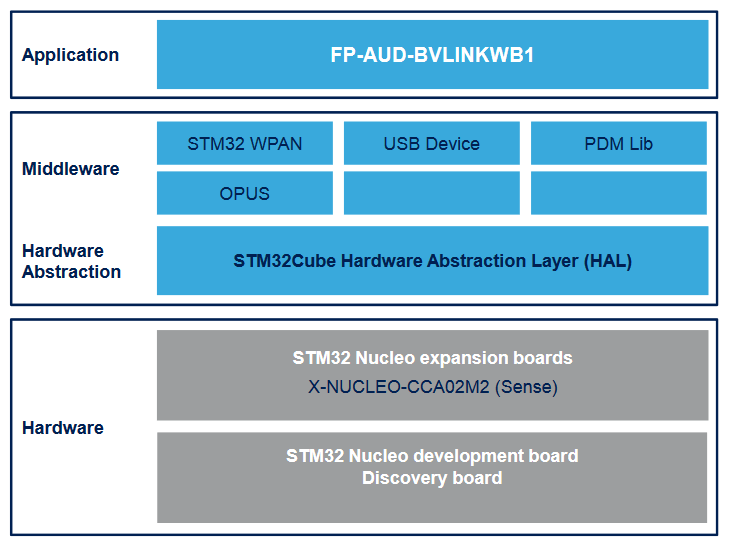
\includegraphics[width=\linewidth]{imgs/firmware_software_arch}
	\caption{Arhitektura softvera FP-AUD-BVLINKWB1}
	\label{fig:firmware_software_arch}
\end{figure}

Komponente za obradu funkcijskog paketa \textit{FP-AUD-BVLINKWB1} dizajnirane su za stvaranje bežične audio veze između modula odašiljača (Tx) i prijemnika (Rx), gdje mikrokontroler služi kao odašiljač, a računalo kao prijemnik. Cijeli lanac obrade zvuka počinje prijemom MEMS digitalnim mikrofonom i kulminira reprodukcijom zvuka na računalu.

BLE je konfiguriran za slanje paketa s maksimalnom veličinom od 150 bajtova. Ovisno o aplikaciji, kodirani bajtovi mogu biti iznad ovog praga, stoga komprimirani međuspremnik (engl. \textit{buffer}) mora biti podijeljen u više BLE paketa. Štoviše, veličina kodiranog međuspremnika može promijeniti svaki audio okvir i prijemnik mora znati njegovu duljinu da bi ga obnovio; za ovaj opseg implementiran je jednostavan protokol BLE prijenosa.

Na strani odašiljača, zvuk se dobiva digitalnim MEMS mikrofonom kao 1-bitni PDM signal i pretvara se pomoću filtra za pretvorbu PDM-u-PCM u 16-bitni PCM. Svaki put kad je audio okvir spreman, prenosi se u algoritam kompresije: veličina kodiranog međuspremnika koju vraća Opus koder može se značajno promijeniti u skladu s parametrima Opus kodera.

\subsection{Opus}
Opus je otvoren i svestran audio kodek koji se može koristiti za različite vrste aplikacija kao što su \textit{streaming} govora i glazbe ili komprimirana pohrana zvuka. Skalabilnost, od uskopojasnog govora niske brzine prijenosa pri 6 kbit/s do stereo glazbe pri 510 kbit/s niske složenosti, čini ga pogodnim za širok raspon interaktivnih aplikacija.

Sastoji se od dva sloja: jedan se temelji na linearnom predviđanju (LP), a drugi se temelji na modificiranoj diskretnoj kosinusnoj transformaciji (MDCT). Opus kombinira rezultate s gubitcima i bez gubitaka. Na primjer, u govornim aplikacijama, LP tehnike poput CELP-a (engl. \textit{Code-excited linear prediction}) učinkovitije kodiraju niske frekvencije nego u tehnikama transformacijske domene kao što je MDCT.

Opus kodek se sastoji od SILK i CELT tehnologija kodiranja. Prvi koristi model temeljen na predviđanju (LPC), dok je drugi u potpunosti modeliran na MDCT transformaciji. Ova svestranost omogućuje Opusu rad u tri načina rada (SILK, CELT ili hibridni način) i osigurava višestruke konfiguracije za različite aplikacije.

\section{Programska potpora za računalo}
BlueST SDK